% kapitel2.tex
%\chapter{Die Softwarekonstruktion}
%\label{chapter:kap2}
\section{Aufbau der Softwarearchitektur}
\label{sec:softwarearchitektur}
Wie im ersten Teil der Ausarbeitung verdeutlicht wurde, ist der Raspberry Pi im Inneren des Spiegels das Kernstück der gesamten Plattform. Auf dieser Hardwarekomponente läuft dementsprechend die komplett entwickelte Software. 

Das Softwareprojekt selbst ist in zwei Komponenten aufgeteilt. Die erste Softwarekomponente realisiert die eigentliche SmartMirror-Anwendung inklusive der Ausgestaltung der Benutzungsschnittstelle, der Kommunikation mit verbauten Sensoren und des Datenimportes aus Datenquellen des Internets. Diese Anwendung ist in Python geschrieben, realisiert die SmartMirror-Funktionalität und hat den größten Anteil des Implementierungsaufwandes erfordert. Im Gegensatz dazu steht die zweite Softwarekomponente, im folgenden StartUp-Anwendung genannt, die ein Skript umfasst, das nach dem Systemstart die SmartMirror-Anwendung startet. Bei dieser handelt es sich um eine erforderliche Hilfskomponente von geringerem Umfang, die als Bash-Skript direkt ausführbar auf Betriebssystemebene realisiert wurde.  

\begin{figure}
	\centering
	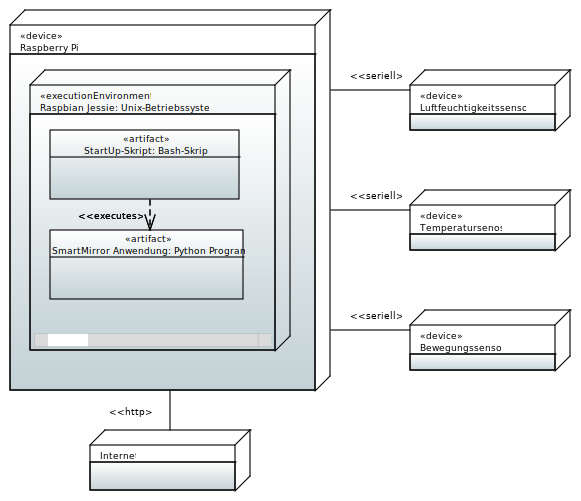
\includegraphics[width=0.8\linewidth]{bilder/DeploymentDiagram}
	\caption[Verteilungsdiagramm der SmartMirror-Applikationen]{Verteilungsdiagramm der SmartMirror-Applikationen}
	\label{fig:verteilungsdiagramm}
\end{figure}

Zum besseren Verständnis ist in \autoref{fig:verteilungsdiagramm} der softwaretechnische Technologiestack der beiden Softwarekomponenten in Form eines UML-Verteilungsdiagramms dargestellt \cite{booch1999uml}. Die zentrale physikalische Ausführungseinheit ist der Raspberry Pi. Dieser kommuniziert über das Serial IO-Protokoll (SIO) mit den zwei verbauten Sensoren: einem Bewegungssensor, sowie einem kombinierten Temperatur- und Luftfeuchtigkeitssensor. Beide Sensoren wurden so gewählt, dass eine Kommunikation über SIO möglich ist. Dieses Protokoll lässt sich über die Adafruit-API sehr gut in Python-Anwendungen einbinden, wie im Unterkapitel \autoref{subsec:strukturAnwendung} weiter ausgeführt wird \cite{adafruit2017}. Des weiteren zeigt das Diagramm, dass zwei weitere Informationsquellen über das Internet, also das http(s)-Protokoll, angebunden werden. Dabei handelt es sich zum Einen um  
einen Newsserver, über den aktuelle T-Online-Nachrichten über einen RSS-Feed eingebunden werden können und zum Anderen um die Einbindung eines Google-Kalenders\cite{feedparserLib}\cite{vayssiere2004system}. Die Kalendereinträge werden über  REST-Webservices im JSON-Format abgefragt\cite{bricalliweb}\cite{bray2014javascript}. 

Die beiden Softwarekomponenten des SmartMirrors laufen auf Basis eines Linux Raspbian Jessie, das als Betriebssystem auf dem Rasberry Pi installiert wurde. Die SmartMirror-Anwendung \glqq SmartMirror.py \grqq ist ein Artefakt, welches durch den Python-Interpreter interpretiert wird. Das StartUp-Skript kann durch direktes Aufrufen der Datei auf dem Betriebssystem ausgeführt werden. 

Beide Softwarekomponenten werden im Folgenden detaillierter beschrieben: zuerst die SmartMirror-Anwendung und dann das StartUp-Skript.

\begin{figure}
	\centering
	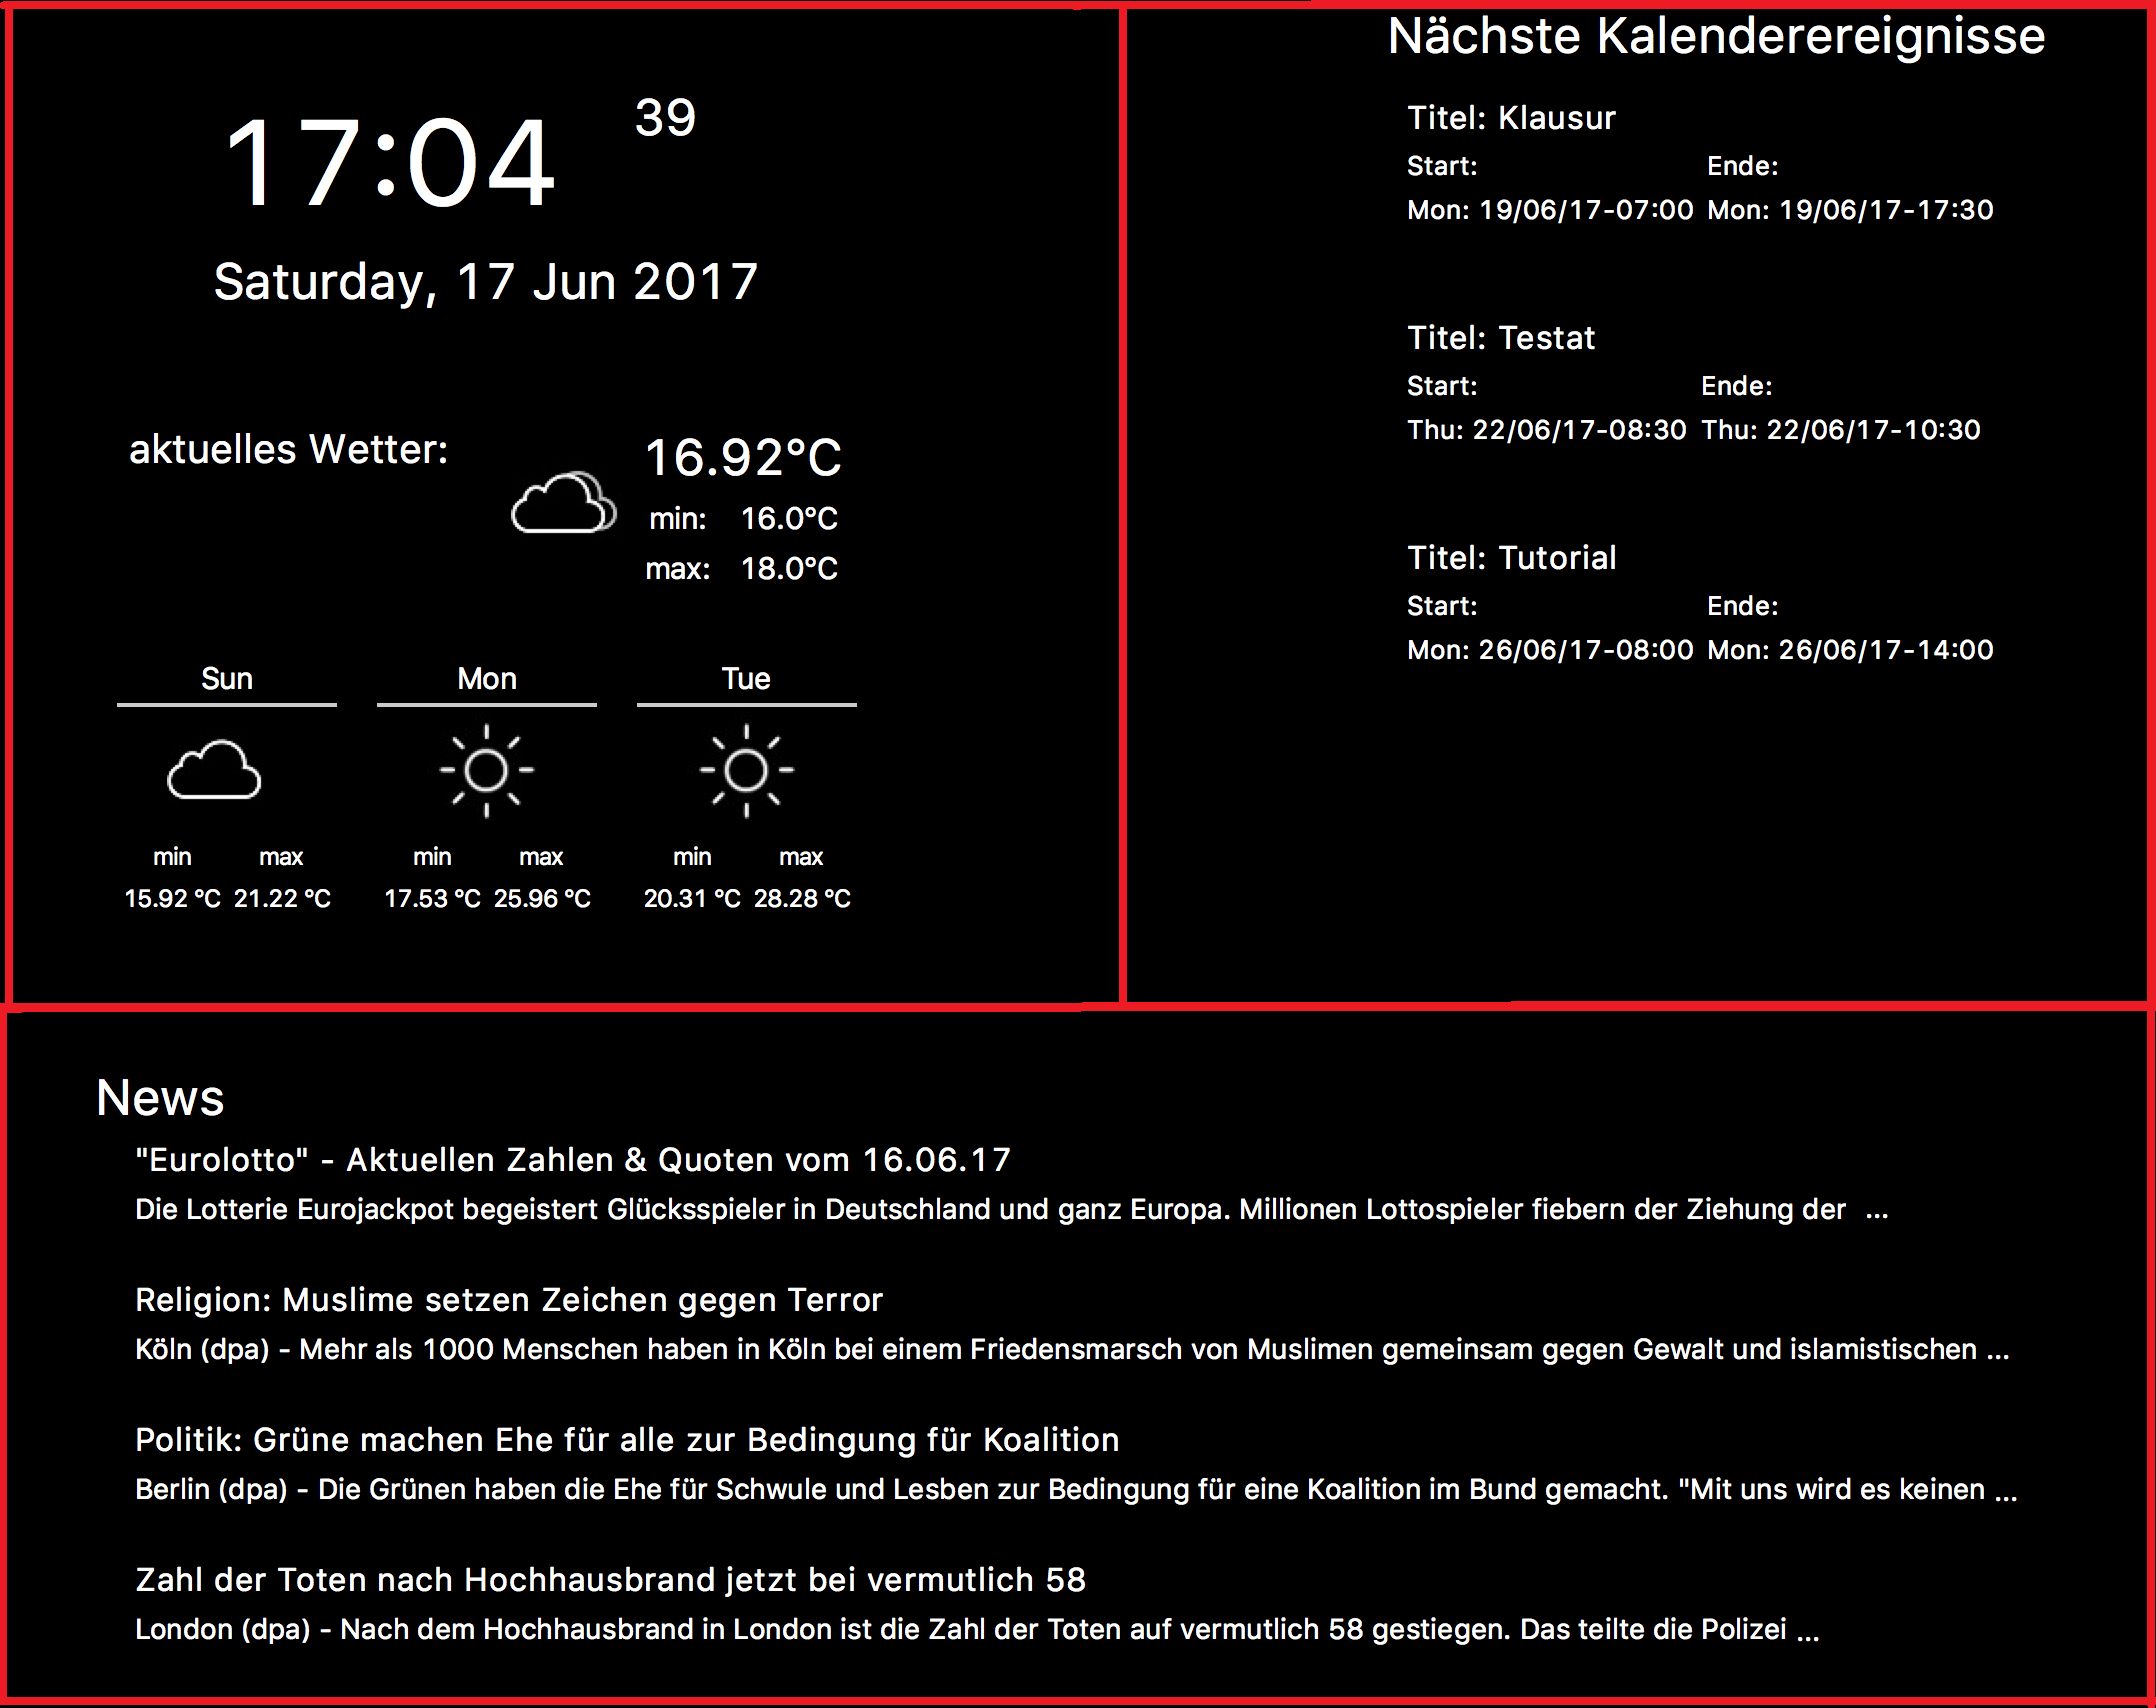
\includegraphics[width=0.8\linewidth]{bilder/grafOberflaeche}
	\caption[Benutzungsschnittstelle der SmartMirror-Anwendung]{Benutzungsschnittstelle der SmartMirror-Anwendung}
	\label{fig:grafoberflaeche}
\end{figure}


\subsection{Die SmartMirror-Anwendung}
\label{smartMirror}
Die Funktionalität der SmartMirror-Anwendung lässt sich am besten ausgehend von der Gestaltung der Benutzungsschnittstelle erfassen, die in \autoref{fig:grafoberflaeche} dargestellt wird. Die Darstellung lässt sich grob in drei Bereiche strukturieren: den oberen linken Bereich, den oberen rechten und den unteren Bereich. Oben links werden aktuelle Informationen konkret Uhrzeit, Datum und Wetterdaten angezeigt, während im rechten Bereich die nächsten Kalenderereignisse aufgeführt werden und im unteren Bereich aktuelle Neuigkeiten (News) angezeigt werden. 

\subsubsection*{Benutzungsschnittstelle}

Zur Gestaltung der Benutzungsschnittstelle wurde das Framework TkInter genutzt. Die Abkürzung steht für (\textbf{Tk Inter}face).  Durch Tkinter ist es mit Python möglich, Programme mit einer grafischen Benutzeroberfläche zu erstellen, die unter Windows, Mac OS und unter einigen Linux-Distributionen laufen. Bei TkInter handelt es sich, um das Standard GUI (Graphical User Interface) Package von Python. Es realisiert eine dünne objektorientierte Schicht über Tcl/Tk \cite{scholl2014tcl}. 

Zur Strukturierung der Oberfläche in die drei zuvor beschriebenen Bereiche wurde der Grid-Manager verwendet. Der Grid-Manager strukturiert Bedienelemente in einer Art Tabelle, die entsprechend in Reihen und Spalten angeordnet ist. Zur Anordnung werden 'row' und 'column' angegeben (vgl. \autoref{lst:structApplication}). Zeile 5 des Listings beschreibt, dass das \textit{GeneralInformation}-Frame, welches Uhrzeit, Datum und Wetterdaten anzeigt, in Zeile 0 und Spalte 0 angeordnet wird und in beide Dimensionen nur eine Zelle benötigt (\textit{rowspan=1, columnspan=1}). Der letzte Parameter in der Zeile (\textit{sticky=\grqq nse\grqq}) definiert die Ausrichtung der Subelement in dem Frame. Dabei steht jedes Zeichen (n, s, e) für eine Himmelsrichtung. Analog dazu wurden in den Zeilen 6 und 7 die weiteren Bereiche auf der Oberfläche angeordnet. In Zeile 7 legt \textit{\textit{columnspan=2}} fest, dass sich der News-Bereich über zwei Spalten erstreckt.

\begin{minipage}{\textwidth}
	\lstinputlisting[frame=single, language=python, style=myPython, escapeinside={(*}{*)}, caption={Hauptklasse der Anwendung}, label=lst:structApplication]{codesnippets/application.py}
\end{minipage}

Jeder Bereich ist als eigenes Frame realisiert. Während sowohl die Kalenderereignisse wie auch die News lediglich eine selbst implementierte Listendarstellung im Frame erfordern, ist das Frame, welches Uhrzeit, Datum und Wetterdaten anzeigt feingranularer strukturiert.

 
\subsubsection*{Struktur der Anwendung}
\label{subsec:strukturAnwendung}
Bei der SmartMirror-Anwendung handelt es sich um eine Drei-Schicht-Architektur (vgl. \autoref{fig:umldiagramClasses})\cite{sharan2015model}. Die Darstellungsschicht (\textit{view}), die zuvor bereits von der Darstellungsseite  beschrieben wurde, greift auf eine weitere Schicht \textit{controller} zu, die alle erforderlichen Daten importiert und in die Datenstrukturen der darunterliegenden Schicht (\textit{model}) speichert.

\begin{figure}
	\centering
	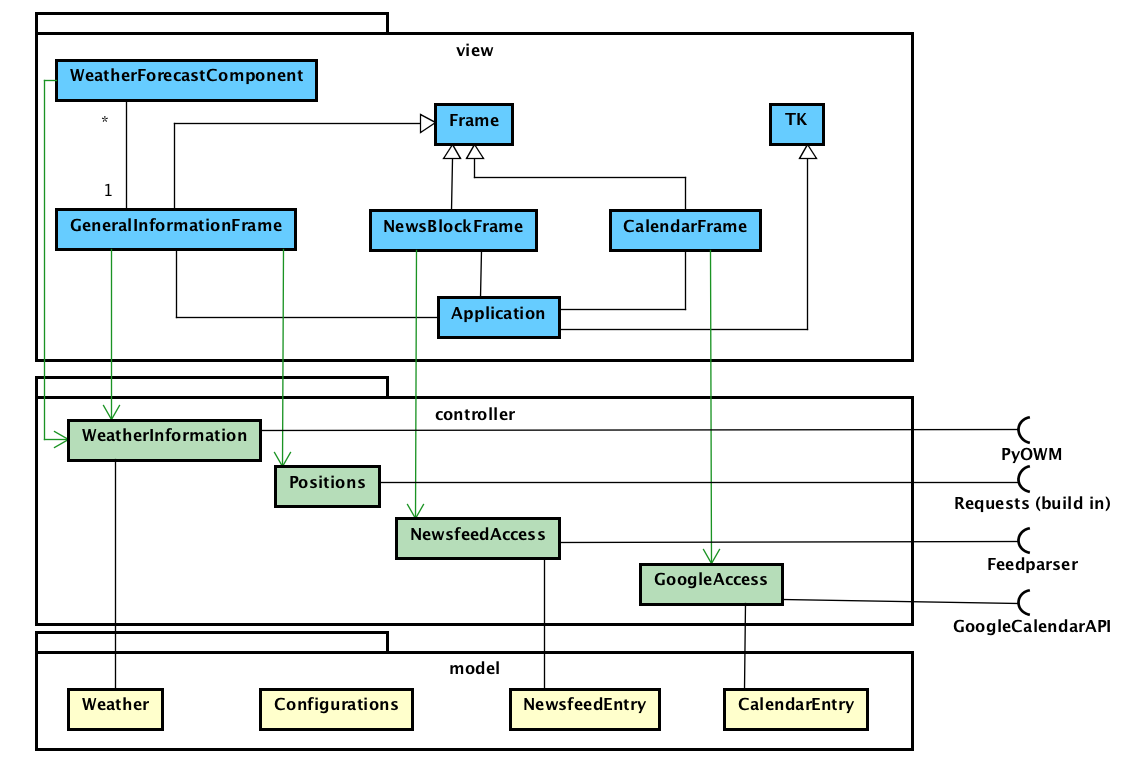
\includegraphics[width=0.8\linewidth]{bilder/umlDiagram_v3}
	\caption[UML-Diagramm: Klassenaufbau der Hauptapplikation]{UML-Diagramm: Klassenaufbau der Hauptapplikation}
	\label{fig:umldiagramClasses}
\end{figure}

Die View-Schicht implementiert als wesentliches Element die Klasse \textit{Application}, die von \textit{Tk} erbt. 
\textit{Application} enthält, wie zuvor erwähnt die Frames \textit{NewsBlockFrame} zur Darstellung von Neuigkeiten, \textit{CalendarFrame} zur Anzeige der nächsten Kalenderereignisse, sowie das \textit{GeneralInformationFrame}. Das \textit{GeneralInformationFrame} nutzt für die Darstellung die \textit{WeatherForeCastComponent}, während die aktuelle Urzeit und das Datum direkt über das Betriebssystem ermittelt und ausgegeben werden. Dies geschieht durch das Kommando \textit{time.strftime(\grq \%H:\%M\grq)} in Zeile 12 (vgl. \autoref{lst:structGeneralFrame}). Hierbei liefert die Methode die aktuelle Uhrzeit in dem Format Stunde:Minute zurück. In der darauf folgenden Zeile wird überprüft, ob sich die aktuell angezeigte Uhrzeit mit der neu Bestimmten übereinstimmt. Ist dies nicht der Fall, so wird in Zeile 14 über das Attribut \textit{$text=new\_ time$} die Aktualisierung vorgenommen.
Zeile 16 sorgt für den erneuten Methodenaufruf nach 200 Millisekunden.

\begin{minipage}{\textwidth}
	\lstinputlisting[frame=single, language=python, style=myPython, escapeinside={(*}{*)}, caption={GeneralInformation Frame},label=lst:structGeneralFrame]{codesnippets/frameExample.py}
\end{minipage}
 
Die Controller-Schicht importiert die anzuzeigenden Daten und bestimmt die aktuelle geographische Position des Spiegels in der Klasse  \textit{Positions}.\textit{Positions} ermittelt über die IP-Adresse des WLAN-Interfaces die Position, um daraus implizit den aktuellen Ort für die Wettervorhersage zu ermitteln. Diese Information benötigt die Klasse \textit{WeatherInformation}, um über die \textbf{Py}thon \textbf{O}pen \textbf{W}eather \textbf{M}ap (PyOWM) die aktuelle Wettervorhersage für den ermittelten Ort anzufragen. PyOWM selbst ist ein Python Wrapper zur Nutzung der Open Weather Map. Die erforderliche Kommunikation zur Ermittlung der Daten ist in (vgl. \autoref{fig:umldiagramClasses}) dargestellt \cite{pyowm}.
 \begin{figure}
 	\centering
 	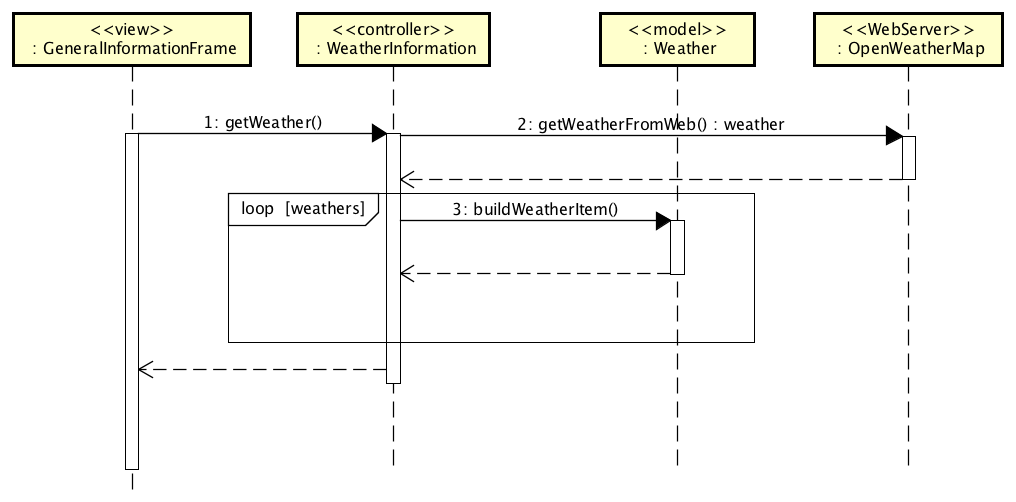
\includegraphics[width=0.8\linewidth]{bilder/sequenceDiagramGettingData_v2}
 	\caption{Sequenzdiagramm: Wetterdaten anfragen vom OWM-Service}
 	\label{fig:sequenzDiagramData}
 \end{figure}

 Die Klasse \textit{GeneralInformationFrame} fordert über die Methode \textit{getWeather} die Wetterdaten von der Klasse \textit{WeatherInformation} an. Diese startet über PyOWM eine Web-Anfrage bei der Open Weather Map. Nach Empfang der Daten legt \textit{WeatherInformation} die Informationen als \textit{Weather}-Daten im Model ab und stellt sie so dem \textit{GeneralInformationFrame} zu Verfügung. 
 Analog fragt die Klasse \textit{NewsfeedAccess} Daten über den Feedparser ab, welcher diese von der \textit{T-Online}-Webseite über einen RSS-Feed bezieht \cite{vayssiere2004system}. Anschließend wandelt der Feedparser die bezogenen Json-Daten in Python-Objekte mit eindeutigen Attributen (\textit{titel}, \textit{description}) um, sodass der Zugriff auf die Nachrichteninhalte implizit vereinfacht wird.
 Ebenso ruft die Klasse \textit{GoogleAccess} die nächsten Kalendereinträge über die GoogleCalendarAPI ab. Dabei wird zur Authentifizierung das O-Auth-Protokoll verwendet, bei dem initial die Berechtigung des Zugriffs auf den Kalender für einen spezifischen Google-Account hinterlegt wird. Anschließend werden analog zu der Open Weather Map Web-Anfragen über die GoogleCalendarAPI erstellt und die empfangenen Daten in ein von Google vorgesehenes Typen-Format konvertiert. \cite{boyd2012getting}
 
 Die Model-Schicht (vgl. \autoref{fig:umldiagramClasses}) speichert Daten, die im SmartMirror angezeigt werden, ebenso wie zentrale Informationen zur Darstellung, die als globale Variablen in \textit{Configurations} vorgehalten werden. Die Klasse \textit{WeatherInformation} nutzt die Klasse \textit{Weather} der Model-Schicht zur Speicherung der Wetterinformationen. 
 Analog dazu speichert die Klasse \textit{NewsfeedAccess} ihre Daten in Form von \textit{NewsFeedEntries} für den \textit{NewsBlockFrame} und die Klasse \textit{GoogleAccess} stellt ihre importierten Daten  als \textit{CalenderEntries} bereit.
 

\subsection{Das StartUp-Skript}
\label{subsec:startup}
Die Funktionalität des \textit{StartUp-Skripts} zeichnet sich durch das Starten der Hauptanwendung aus, nachdem der \textit{Raspberry Pi} mit dem Bootvorgang fertig ist. Dazu wurde ein Bash-Skript (vgl. \autoref{lst:startup}) geschrieben, welches automatisch beim Starten des Computers ausgeführt wird. 
Das direkte Ausführen des Skripts wird dadurch realisiert, dass die Datei in das Verzeichnis \textit{/etc/init.d/} gelegt wird, wodurch sie direkt im Anschluss an die Bootsequenz ausgeführt wird. \cite{nemeth2006linux}

\begin{minipage}{\textwidth}
	\lstinputlisting[language=bash, frame=single, caption={StartUp-Skript}, label=lst:startup]{codesnippets/startscript.sh}
\end{minipage} 

Das Skript ist recht einfach aufgebaut. In der ersten Zeile wird das Interpreter-Programm \textit{/bin/sh} definiert, womit das Skript ausgeführt wird. Als nächstes wechselt das Kommando in Zeile 3 in das Verzeichnis der \textit{SmartMirror}-Anwendung (vgl. \autoref{smartMirror}), um die Anwendung dort in Zeile 5 zu starten. Die Zeile 4 stellt ausschließlich sicher, dass der Hauptmonitor für den grafischen Output verwendet wird, damit die UI der \textit{SmartMirror}-Anwendung auch in dem Spiegel dargestellt wird. Wenn diese Zeile ausgelassen würde und der Raspberry Pi ohne GUI startet, dann läuft zwar die Anwendung für den Spiegel, aber weil kein grafischer Ausgang definiert ist, wird die Anwendung nicht auf dem externen Monitor visualisiert. Somit bietet die Zeile eine Sicherheit, dass auch wirklich ein angeschlossener Monitor angesteuert wird.

\section{Der SmartMirror im Einsatz}

Sobald die beiden Teilkonstruktionen \autoref{sec:hardwarekonstruktion} und \autoref{sec:softwarearchitektur} miteinander verknüpft werden, entsteht das in \autoref{fig:spiegelfertig} dargestellte Ergebnis.
Um jedoch die Software auf die Hardware zu überspielen, sodass die Software auch stabil läuft, sind Zwischenschritte nötig, die im Folgenden detaillierter beschrieben werden.

So ist als erstes dafür zu sorgen, dass der Raspberry mit dem Internet verbunden ist, um benötigte Software installieren zu können. Anschließend ist sicherzustellen, dass die richtige Version von Python (3.6) und damit des Python-Interpreters installiert ist, da sonst die \textit{SmartMirror}-Anwendung nicht ausgeführt werden kann. 
Außerdem müssen alle bei der Implementierung integrierten Libraries, ebenfalls auf dem Raspberry Pi installiert sein. 
Im letzten Schritt muss noch das StartUp-Skript in den das \autoref{subsec:startup} beschriebene Verzeichnis kopiert werden und in der \textit{Configurations.py} müssen die korrekten GPIO-Pins für die entsprechenden Sensoren hinterlegt werden. 

Nachdem diese Schritte durchgeführt wurden, startet der Spiegel nach einem Neustart direkt mit der softwareseitig Implementieren UI und repräsentiert damit den fertigen Spiegel, der ausschließlich an den Strom angeschlossen und eine zuvor konfigurierte Internetverbindung herstellen muss. 

\begin{figure}
	\centering
	\includegraphics[width=0.8\linewidth]{bilder/spiegelVorneLinks}
	\caption[Fertiger Spiegel inklusive Anzeige der Daten]{Fertiger Spiegel inklusive Anzeige der Daten auf dem Spiegel}
	\label{fig:spiegelfertig}
\end{figure}
